\chapter{Implementazione}
\label{chapter:implementazione}

\section{Processo di Simulazione dello Scenario}

Al fine di valutare le prestazioni degli scenari di Fog Computing, descritti al capitolo \ref{chapter:architettura}, è stato implementato un sistema di simulazione che ne permette in una prima fase la definizione in ogni suo aspetto (topologia, applicazioni, servizi, richieste, ecc...) e, successivamente, l'analisi dei principali aspetti utili alla comprensione dello scenario, come il successo del \textit{service placement} e delle richieste di servizi da parte dei vari nodi della rete.

La definizione e l'esecuzione della simulazione seguono il diagramma di flusso mostrato in Figura \ref{fig:sim_flow_diagram}.

\begin{figure}[!ht]
  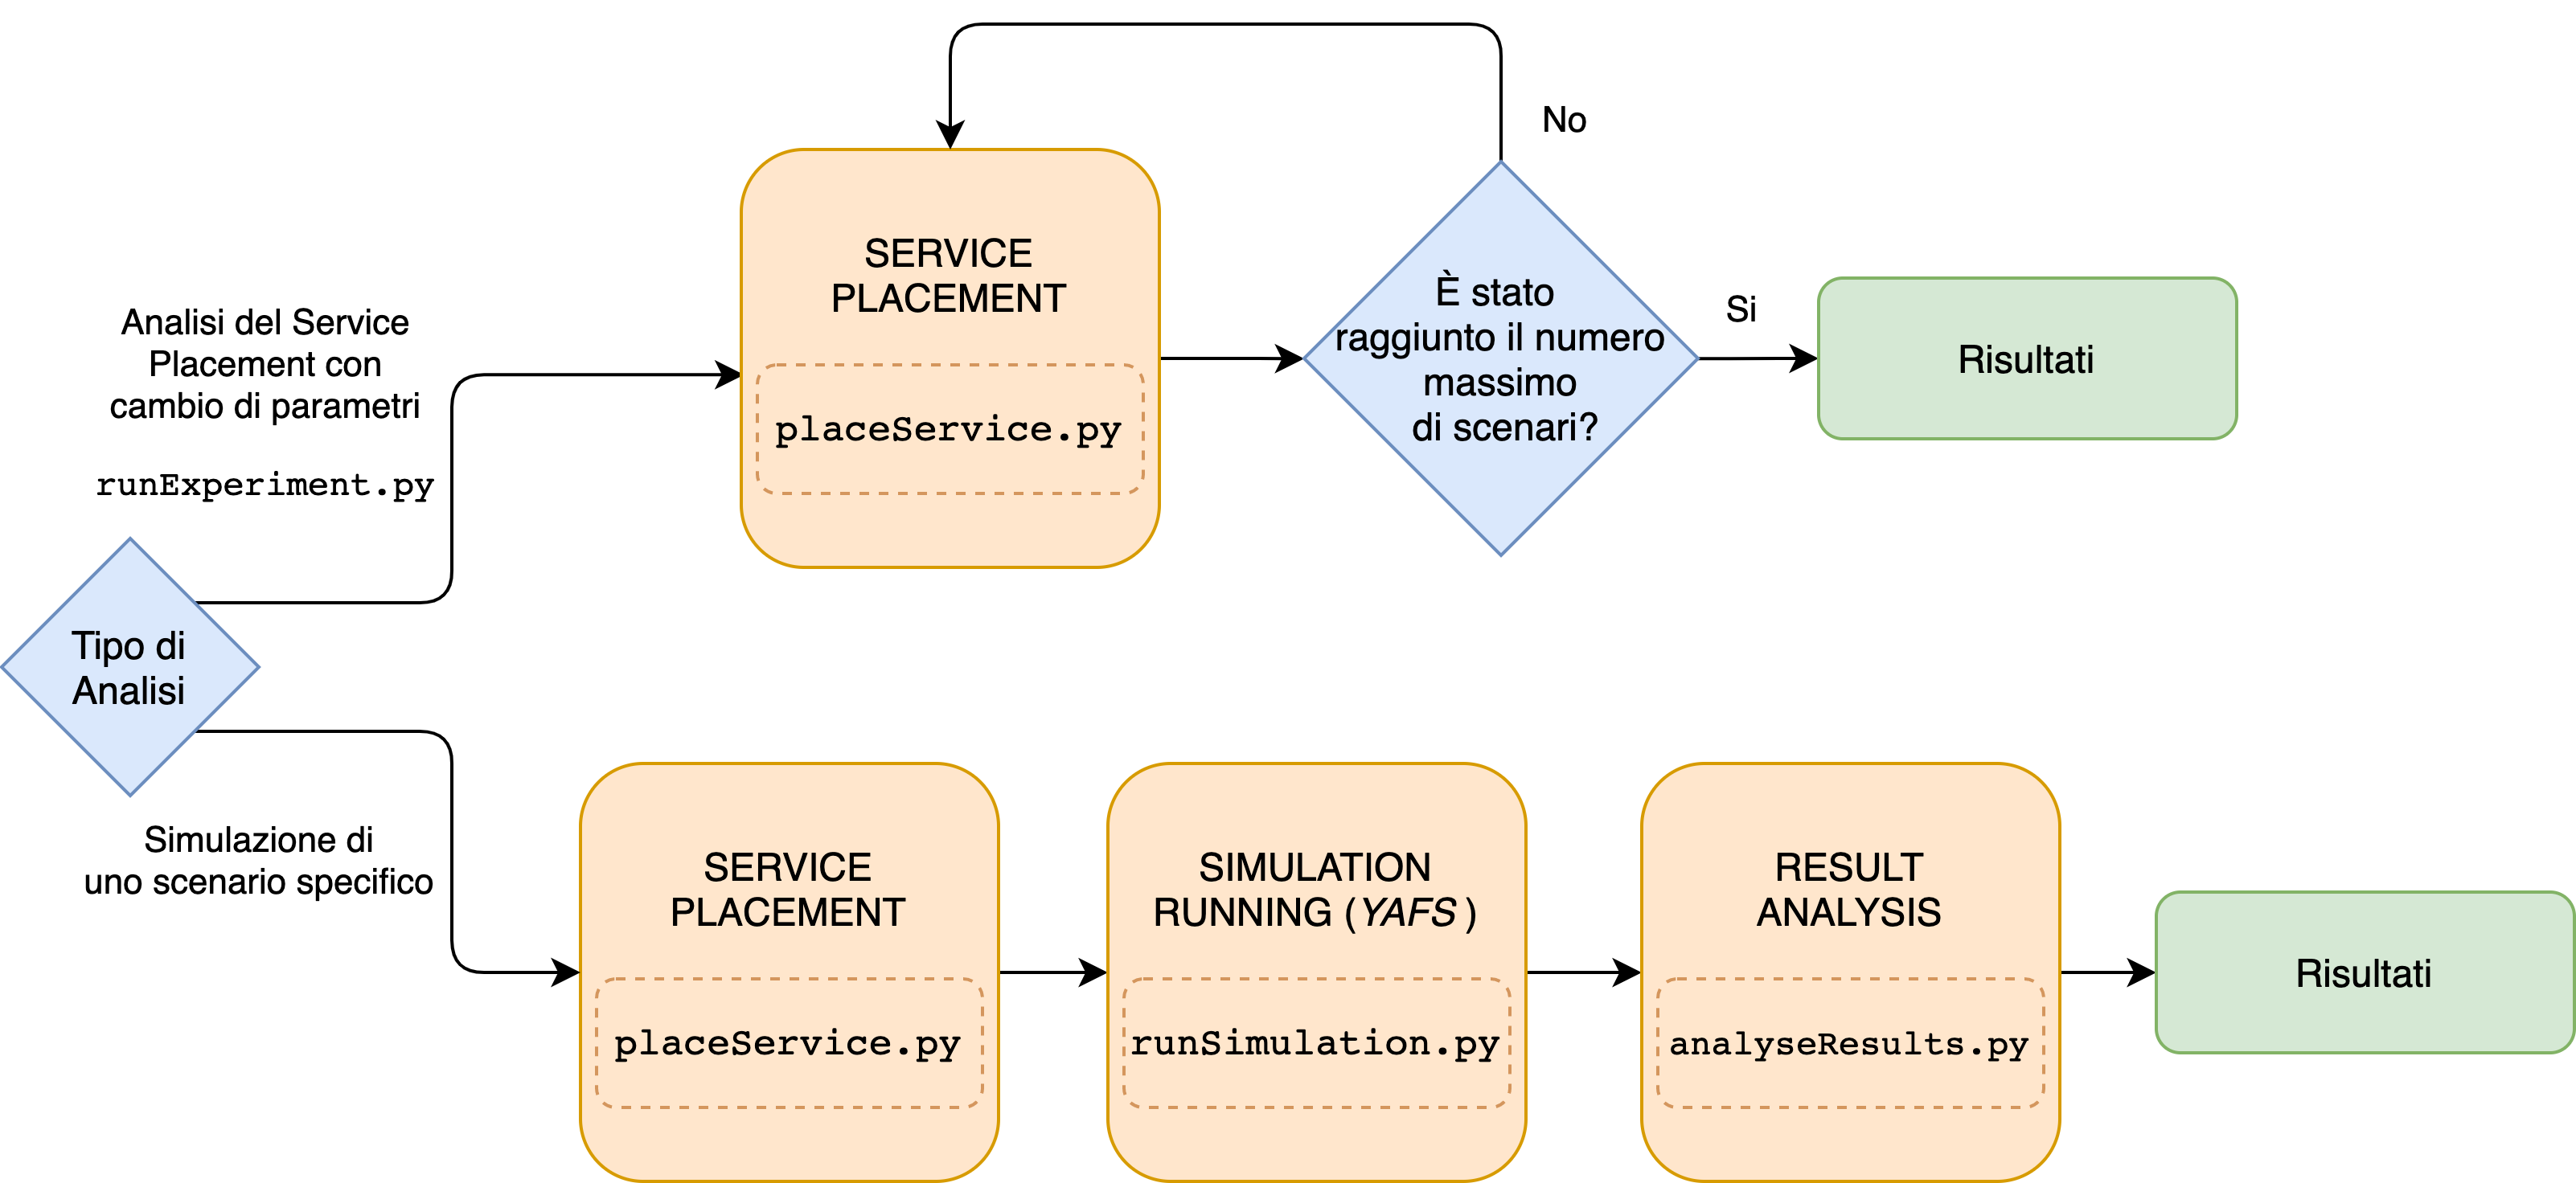
\includegraphics[width=14cm]{images/sim_flow_diagram}
  \centering
  \caption{Tre tipologie di applicazioni realizzabili, con la loro rappresentazione tramite grafo.}
  \label{fig:sim_flow_diagram}
\end{figure}